
\chapter{Results} \label{chap-results}

\bigskip

This chapter presents the results of the methods described in Chapter \ref{chap-meth}. We begin with Section \ref{res-cor-stat} which presents the filtering method results and the scope of the network that will be further analyzed. Section \ref{sec-res-buff} presents the extended filter and the further reduction of the networks.


%%%%%%%%%%%%%%%%%%%%%%%%%%%%%%%%%%%%%%%%%%%%%%%%%%%%%%%%%%%%%%%%
% \section{Feature Importance Exploration}\label{res-feature}
% glmnet
% rf
% pca

% Using the data from the pre-processing stage in Section \ref{sec:meth-processing}


%%%%%%%%%%%%%%%%%%%%%%%%%%%%%%%%%%%%%%%%%%%%%%%%%%%%%%%%%%%%%%%%%%
\section[Initial Correlation and Statistical Significance Filtering]{Initial Correlation and Statistical \\ Significance Filtering}\label{res-cor-stat}

Using the \acrshort{FastSpar} method, we generated fully connected correlation matrices for the control and case data. A heat map visualization of the healthy network can be found in Figure \ref{fig-h-orig-heatmap} and the diseased heat map can be found in the appendix as Figure \ref{apdx-fig-d-orig-heatmap}. The genera in the network are listed on the respective axes, and spaces are colored according to the correlation values present in the matrix. Self-associated connections occur with a correlation strength of 1; as is visible along the diagonal of the heat map. These figures show fully connected correlation networks, so it is necessary for us to filter this initial result for better understanding of the underlying network properties.
\begin{figure}[!htb]
    \centering
    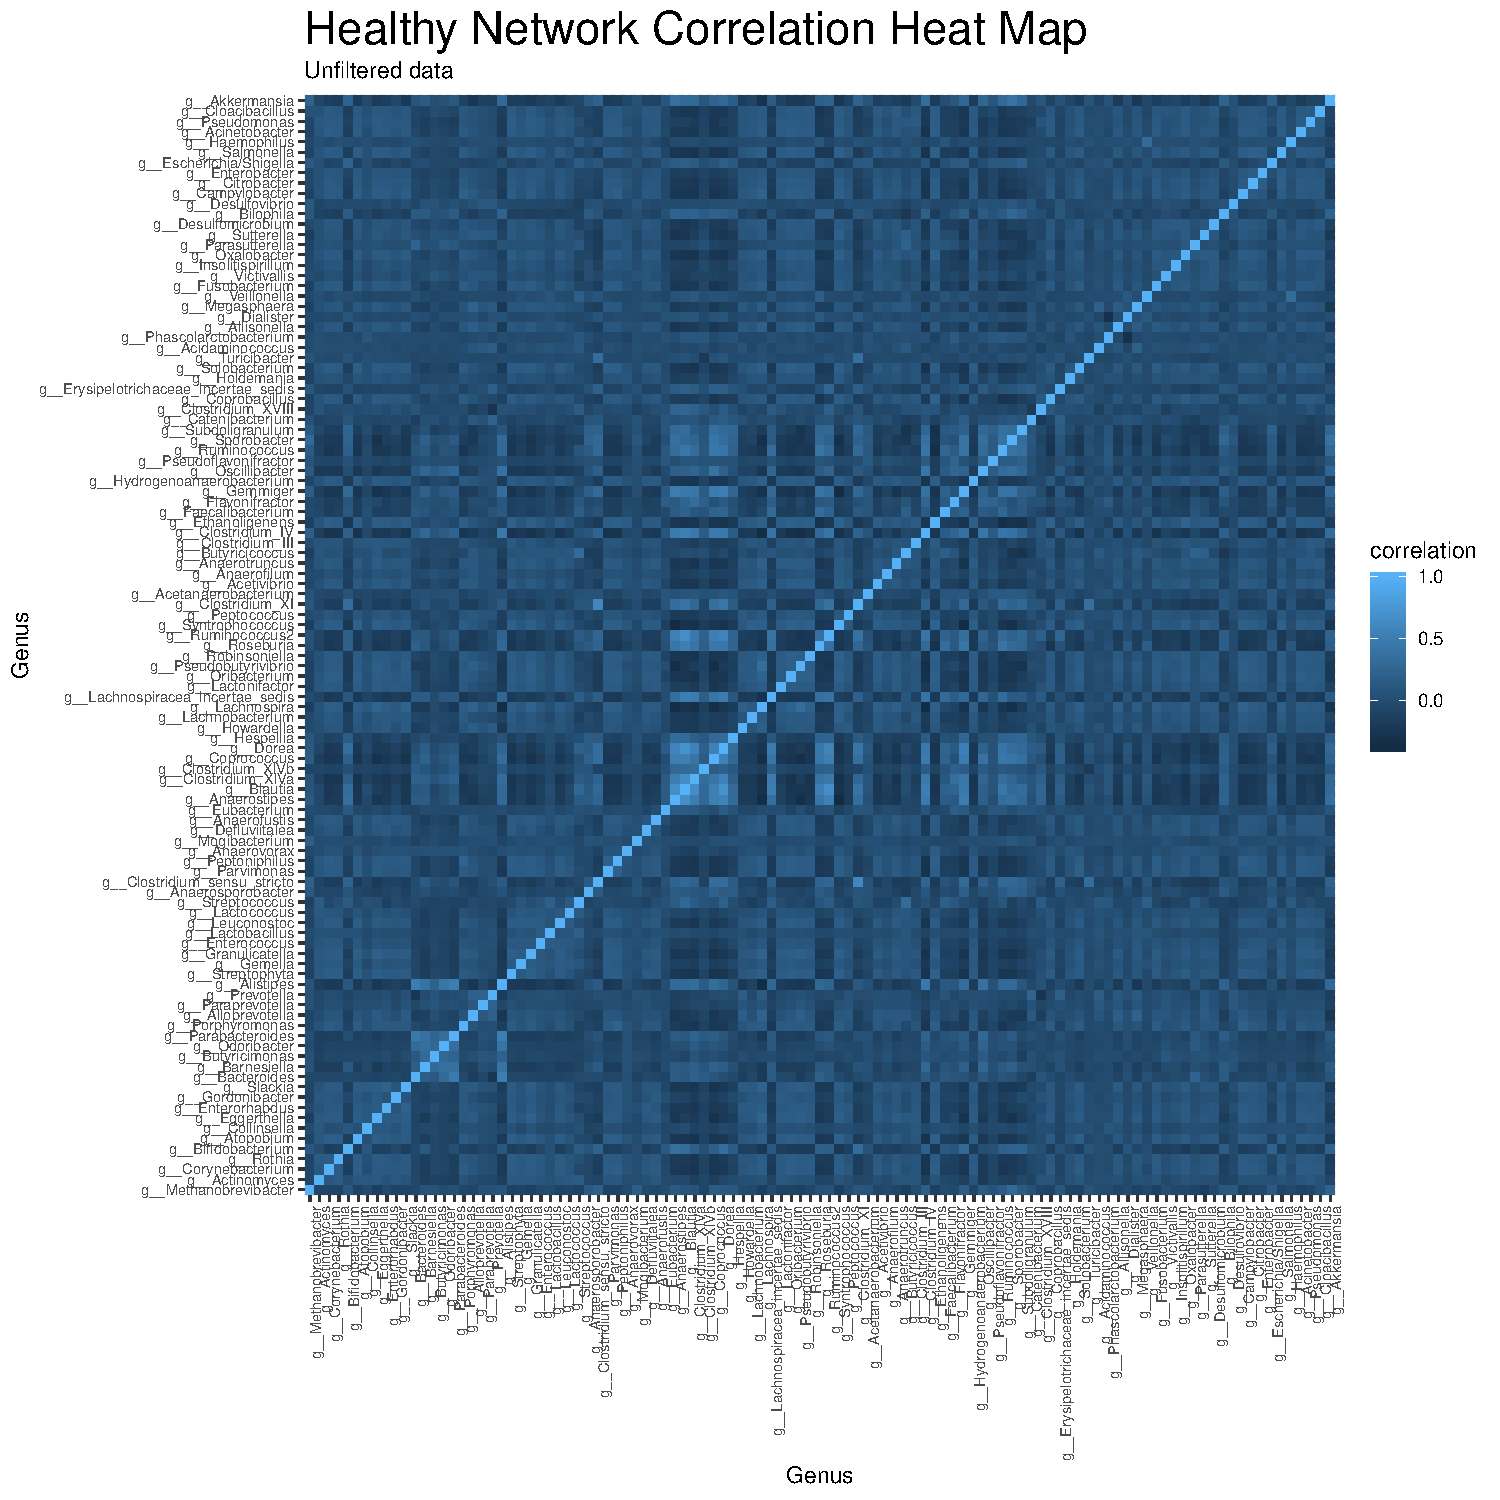
\includegraphics[width=1.0\linewidth]{figure/results/healthy_raw_corr_heatmap.pdf}
    \caption[Heat map of the resulting \acrshort{FastSpar} correlation matrix.]{Heat map of the resulting \acrshort{FastSpar} correlation matrix. Genera are listed on the respective axes and correlation values are colored based upon their strength.}
    \label{fig-h-orig-heatmap}
\end{figure}
 Figures \ref{fig-res-h-dist} and \ref{fig-res-d-dist} present the correlation and $p$-value histograms for the healthy (control) and disease (case) networks with some of the filtering criteria utilized.

 In Figure \ref{fig-res-h-dist}, a majority of the correlation values are significant. In the unfiltered data, the distribution of correlations appears to be close to a normal distribution, with some skew toward 1.0. Almost all of the $p$-values have a value of 0.00001. 107 of these $p$-values were equal to 1, and they were associated with a taxon's self correlation (as mentioned previously with regard to Figure \ref{fig-h-orig-heatmap}). 
 We were not interested in correlations close to 0, nor were we interested in the correlation of a taxa with itself, so in the next row of Figure \ref{fig-res-h-dist} we filtered the data by keeping correlations $|c| \geq 0.25$, but did not filter by the $p$-value. After this step we saw a large reduction in the number of correlation values, as well as $p$-values that were between our smallest and largest values. Filtering at this level consequently has revealed that roughly a quarter of the remaining correlations are associated with $p$-values of 1. We knew that these belong to the self-correlations of the taxa, so we changed our filtering criteria to keep the same correlation filter while adding a filter to keep all $p$-values $p \leq 0.01$ and eliminating the diagonal (of the matrix) self-associated correlations. At this step we significantly reduced the connectivity and size of the network by removing correlation values close to 0 while removing all of the statistically insignificant correlations. We ran many different filtering methods, but this one appeared to be the closest to what we were looking for.
 
 Included in the bottom row of Figure \ref{fig-res-h-dist} is an additional filtering method where we filtered by $p \leq 0.01$ and $c \geq 0.05$. With this filtering method there are still several thousand connections in the network, but all the $p$-values are statistically significant. Since there were still so many correlation values, we must increase the correlation threshold. 

\begin{figure}[!htb]
    \centering
    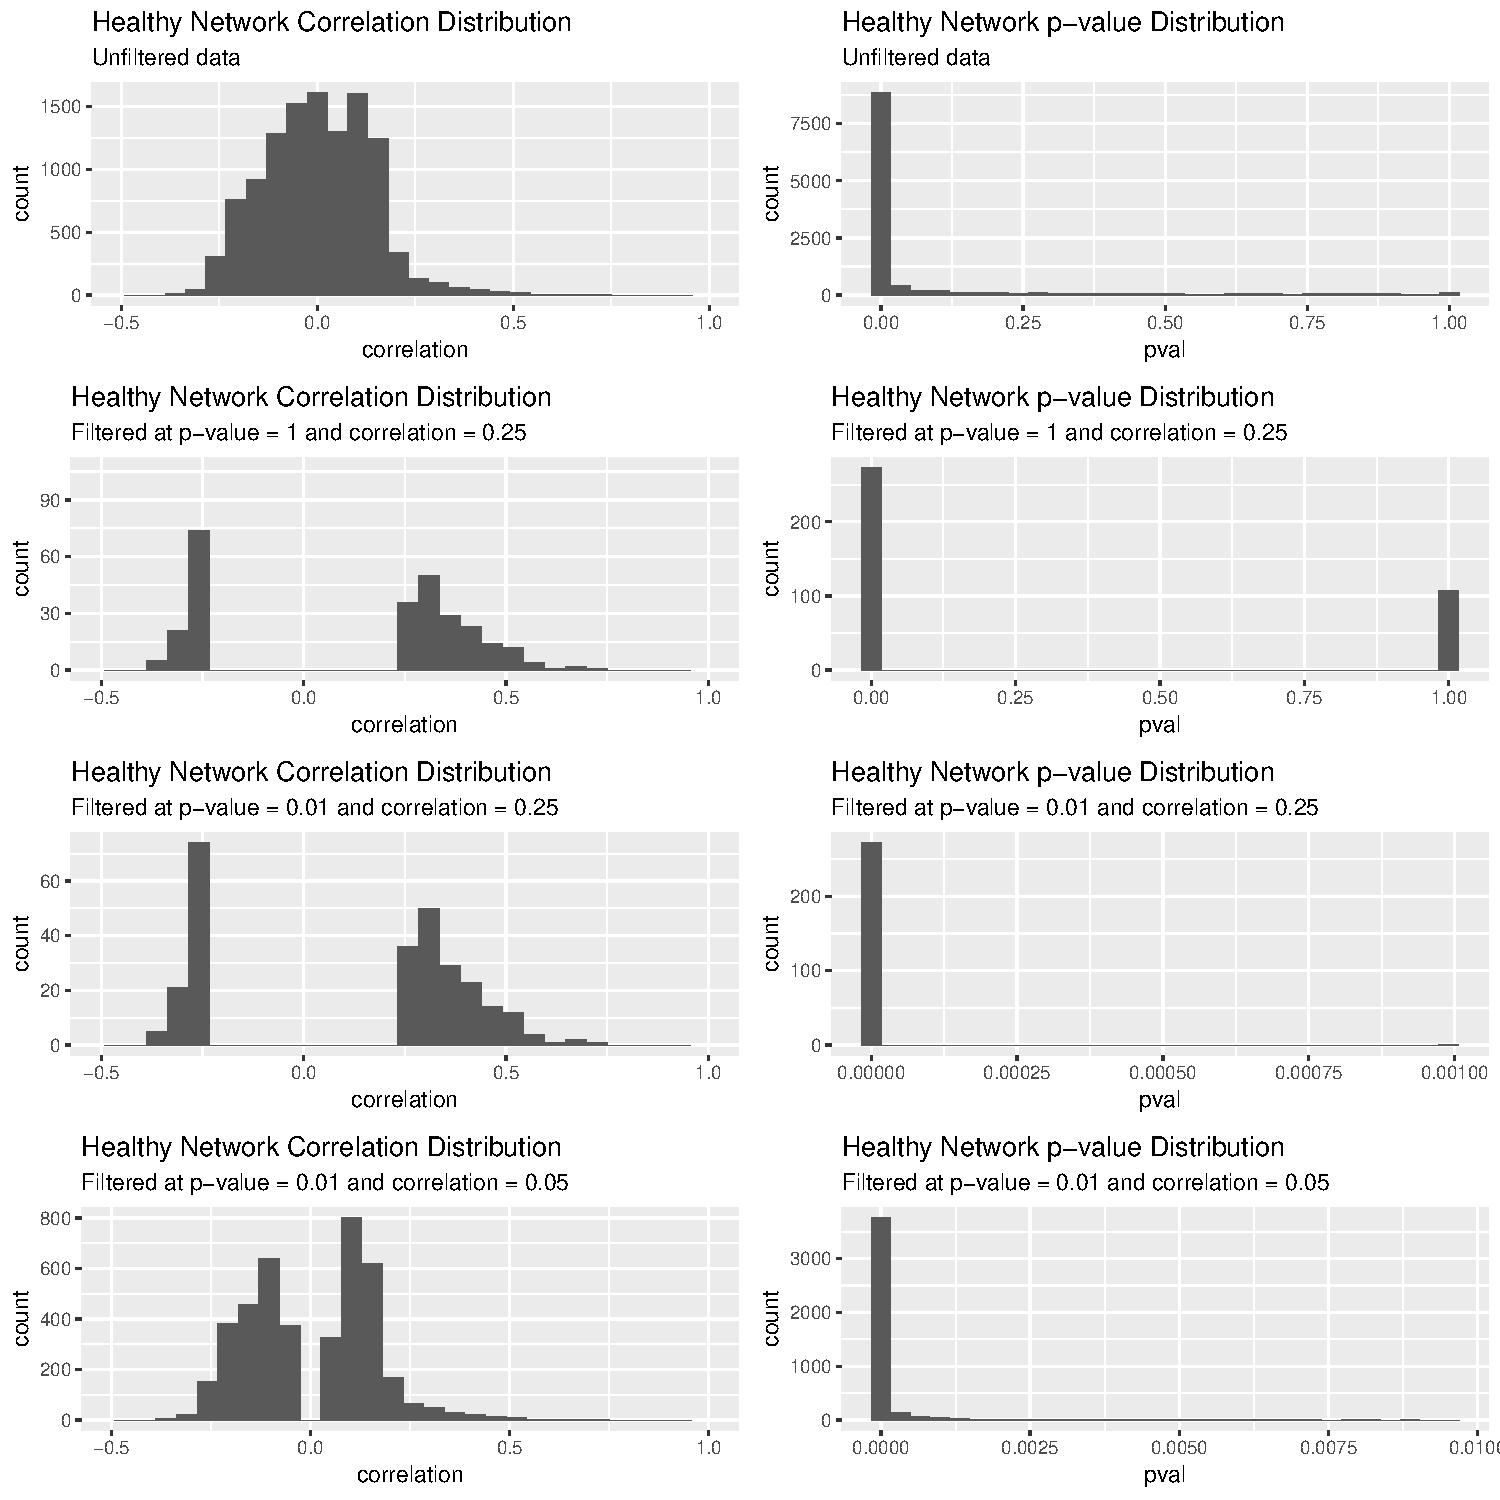
\includegraphics[width=1.0\linewidth]{figure/results/healthy_distributions_corr_pval_dist.pdf}
    \caption[Histogram distribution comparison of the healthy network filtered at varying correlation and $p$-value levels.]{Histogram distribution comparison of the healthy network filtered at varying correlation and $p$-value levels. The chosen parameters selected for visualization include: the raw unfiltered data, the network containing all correlations $c$ where $|c| \geq 0.25$, network with all connections with $p \leq 0.01$ and $|c| \geq 0.25$, and the network with all connections with $p \leq 0.01$ and $|c| \geq 0.05$.}
    \label{fig-res-h-dist}
\end{figure}

\begin{figure}[!htb]
    \centering
    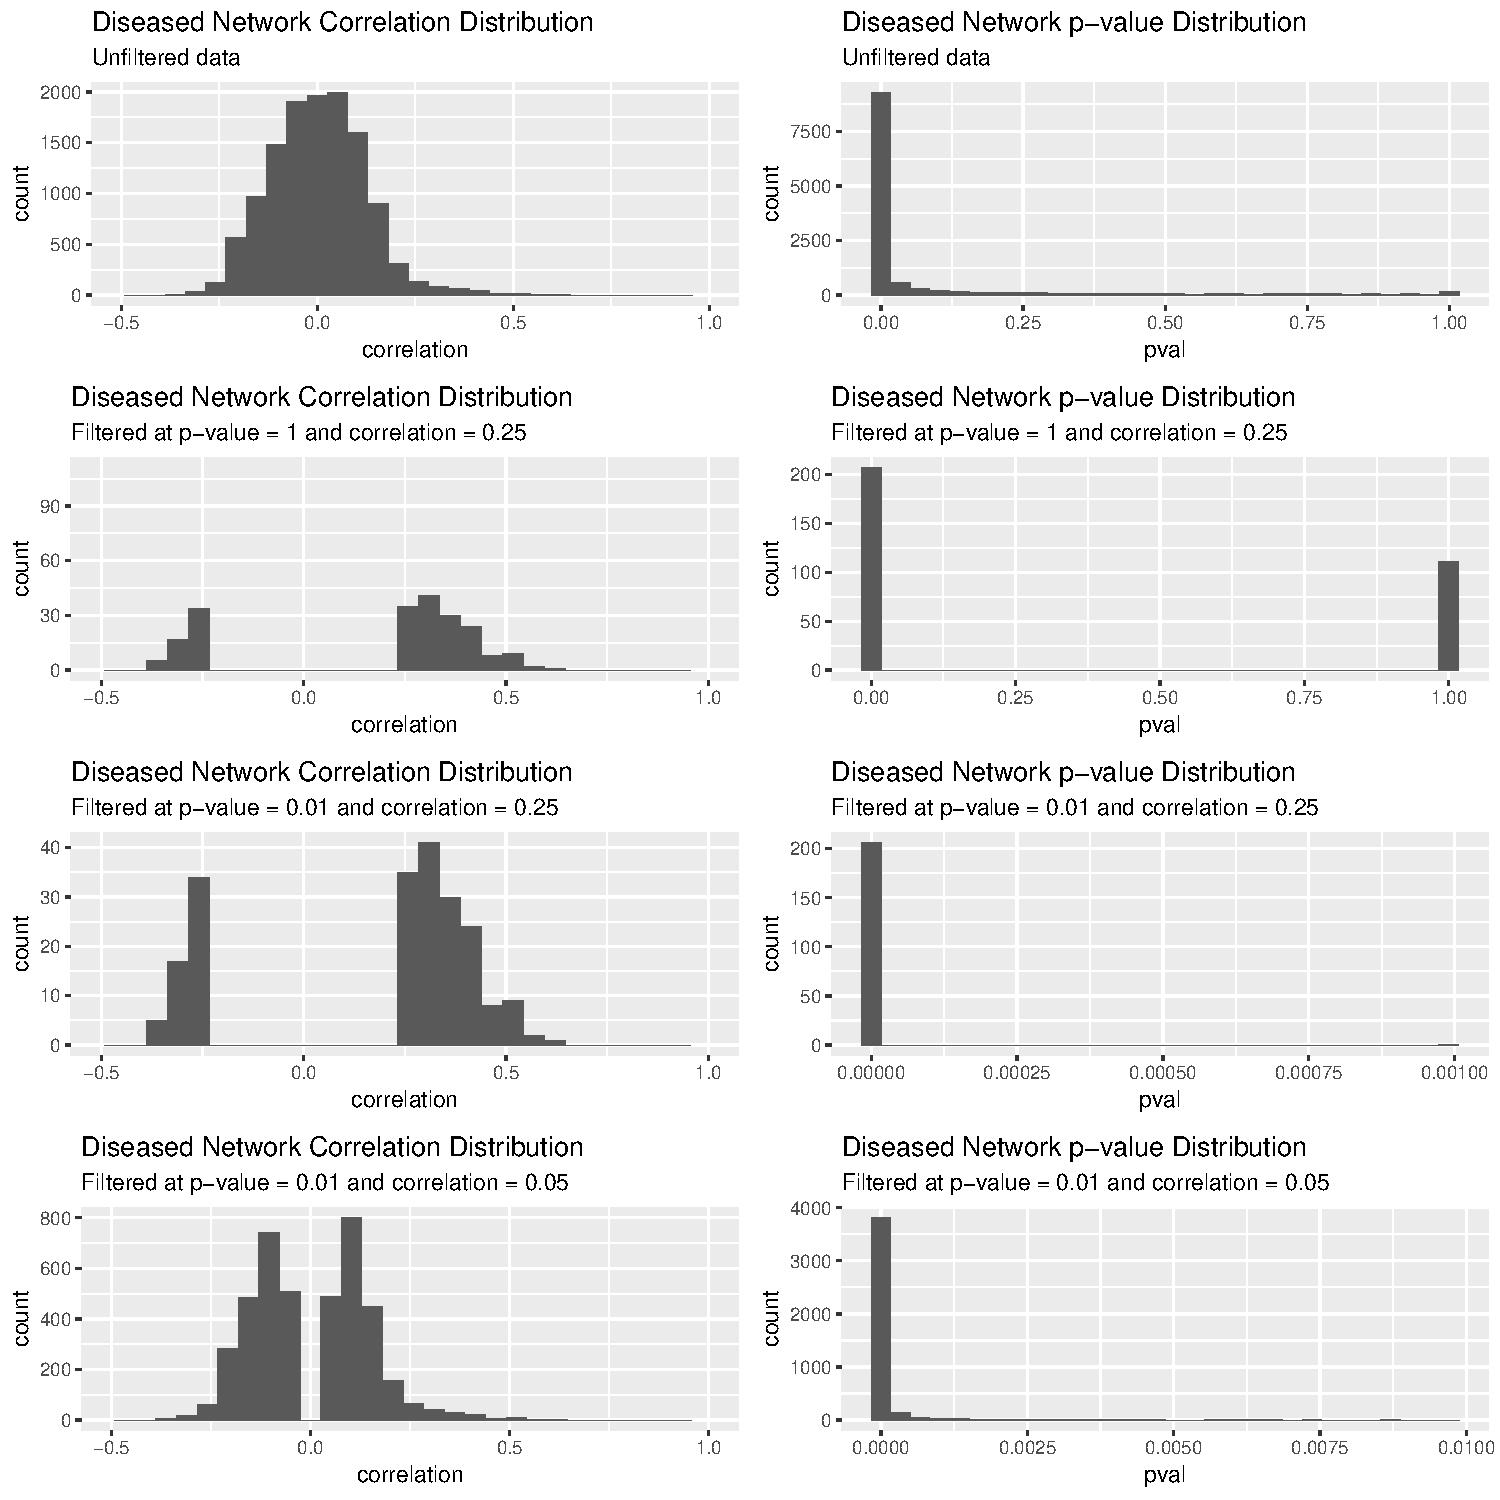
\includegraphics[width=1.0\linewidth]{figure/results/diseased_distributions_corr_pval_dist.pdf}
    \caption[Histogram distribution comparison of the diseased network filtered at varying correlation and $p$-value levels.]{Histogram distribution comparison of the diseased network filtered at varying correlation and $p$-value levels. The chosen parameters selected for visualization include: the raw unfiltered data, the network containing all correlations $c$ where $|c| \geq 0.25$, network with all connections with $p \leq 0.01$ and $|c| \geq 0.25$, and the network with all connections with $p \leq 0.01$ and $|c| \geq 0.05$.}
    \label{fig-res-d-dist}
\end{figure}
The distributions listed in Figure \ref{fig-res-d-dist} are similar to those of the healthy network. We applied the same filtering methods as described before due to the similarity in correlation and $p$-value distributions. In the diseased network there were 111 genera present, and thus 111 self-associated connections were filtered out. We found that by choosing the $p$-value cutoff of $p \leq 0.05$ and the correlation cutoff of $|c| \geq 0.25$ we were able to eliminate a majority of the connections and the remaining connections were all statistically significant. Similar behavior between the networks in this filtering stage suggests that the structure of the two networks is similar and that further comparisons might yield additional results. 

\begin{table}[hbt]
\centering
\begin{tabular}{p{3cm} p{3cm} p{4cm}}
    \toprule
    Cohort Data & Total Edges & Edges After Filter 1 \\ 
    % \midrule
    \midrule
    Healthy & 5671 & 272 \\ 
    Diseased & 6105 & 206 \\ 
   \bottomrule
\end{tabular}
\caption[Table including the total edges before and after the first filter.]{Table including the total edges before and after the first filter. We first found the total edges in each cohort by only looking at the upper triangle of the respective matrix. We then filtered with the 0.25 correlation threshold and the $p$-value threshold of 0.01. }
\label{tab:edge_table1}
\end{table}
Table \ref{tab:edge_table1} describes the number of edges before and after applying the initial filter. There were a total of 5671 and 6105 unique edges for the healthy and diseased networks respectively. After the first round of filtering there were 272 and 206 edges respectively. Despite there being more connections in the diseased network prior to filtering, the first filtering step yielded more healthy edges.

\section{Extended Correlation Filtering}\label{sec-res-buff}
% Summing the Edges After Filter 1 components in Table \ref{tab:edge_table1} with the respective entries in the Overlapping Edges Added from Filter 2 column in this table sums to the Total Edges with Filter 1 and Filter 2.

In Section \ref{meth:filtering} we mentioned the implementation of an extended correlation filter for the correlation values close to the original filter's threshold. We found the shared connections between the filtered healthy network and unfiltered diseased network and sorted them by correlation difference as demonstrated in Figure \ref{subfig:all_buff_h}. We performed the same method for the filtered diseased network and unfiltered healthy network in Figure \ref{subfig:all_buff_d}. In the figures, connections that are the most similar are on the left and those that have the largest difference are on the right. It is interesting to note that as we traverse right toward larger correlation differences the unfiltered network's correlations tend to converge towards 0. Unfortunately we do not compare these parts of the networks if the unfiltered values do not meet the extended filter criteria. Additionally, we do not compare these components because of our use of the \acrshort{NESH} score. Recall that it is a value contingent on the overlapping sub-graphs of the two networks. Both Figure \ref{subfig:all_buff_h} and \ref{subfig:all_buff_d} demonstrate that filtering should be employed to significantly reduce the large amount of noisy data visible in the figures.

\begin{figure}[!hbt]
\centering
\subfloat[Shared edges with the healthy network as the filtered network, and diseased as unfiltered.]{
    \label{subfig:all_buff_h}
    \fbox{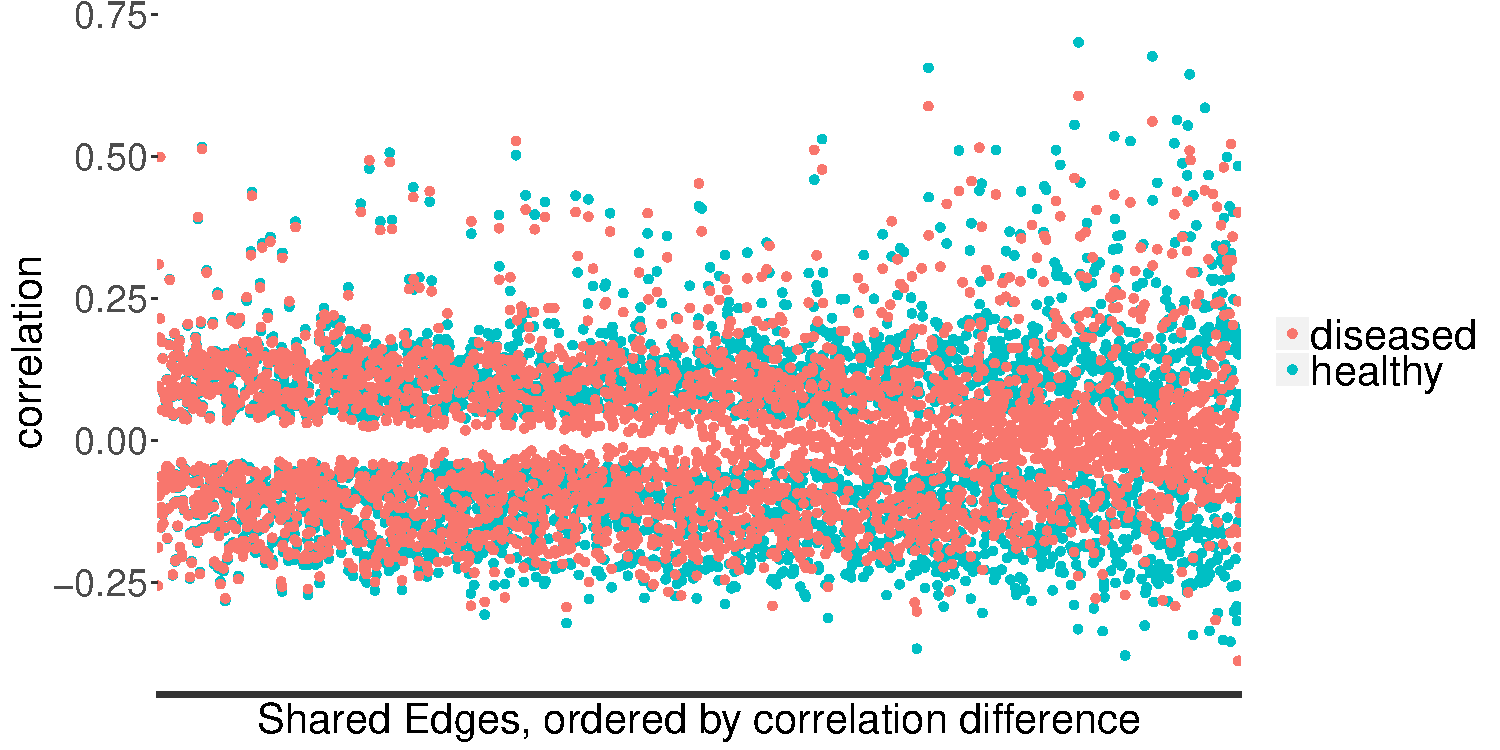
\includegraphics[width=0.8\textwidth]{figure/results/correlation_comparison_h_all.pdf}}}
    \hfill
\subfloat[Shared edges with the diseased network as the filtered network, and healthy as unfiltered.]{
    \label{subfig:all_buff_d}
    \fbox{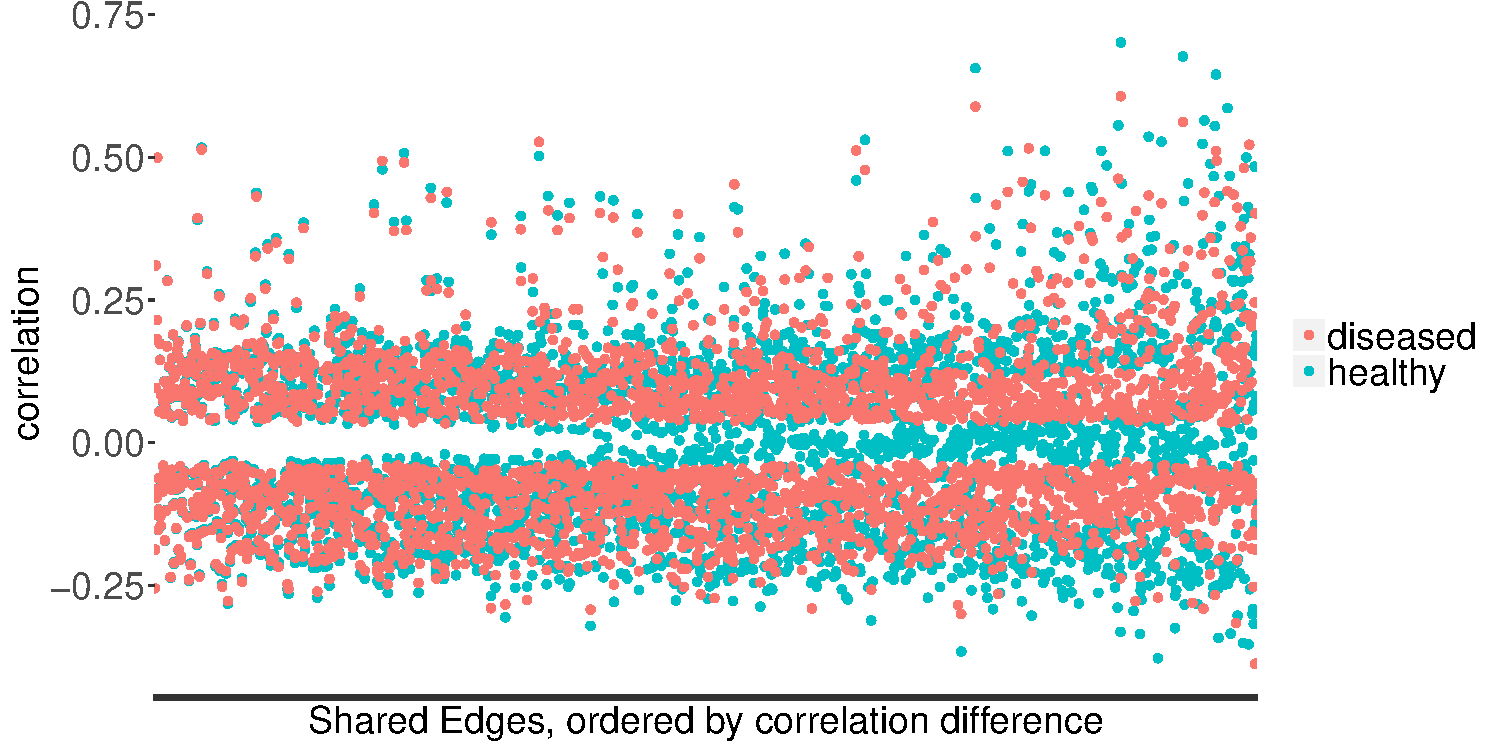
\includegraphics[width=0.8\textwidth]{figure/results/correlation_comparison_d_all.pdf}}}
\caption{All shared connections between the healthy and diseased networks. In each case the filtered network had all correlation values equal to 0 removed, and all edges with $p$-values greater than 0.05 were removed as well. }
\label{fig:buffer-all}
\end{figure}

When comparing the two sub-figures in Figure \ref{fig:buffer-all} we saw a significant number of correlations close to 0 in both filtered and unfiltered networks. Following our results in the previous section, we removed a majority of the correlation values that lead to the fully connected matrices despite being close to 0. It appeared that selecting a correlation value threshold of $\pm 0.25$ allowed us to ignore a majority of the low-value correlations.
% \begin{figure}[!hbt]
%     \centering
%     \fbox{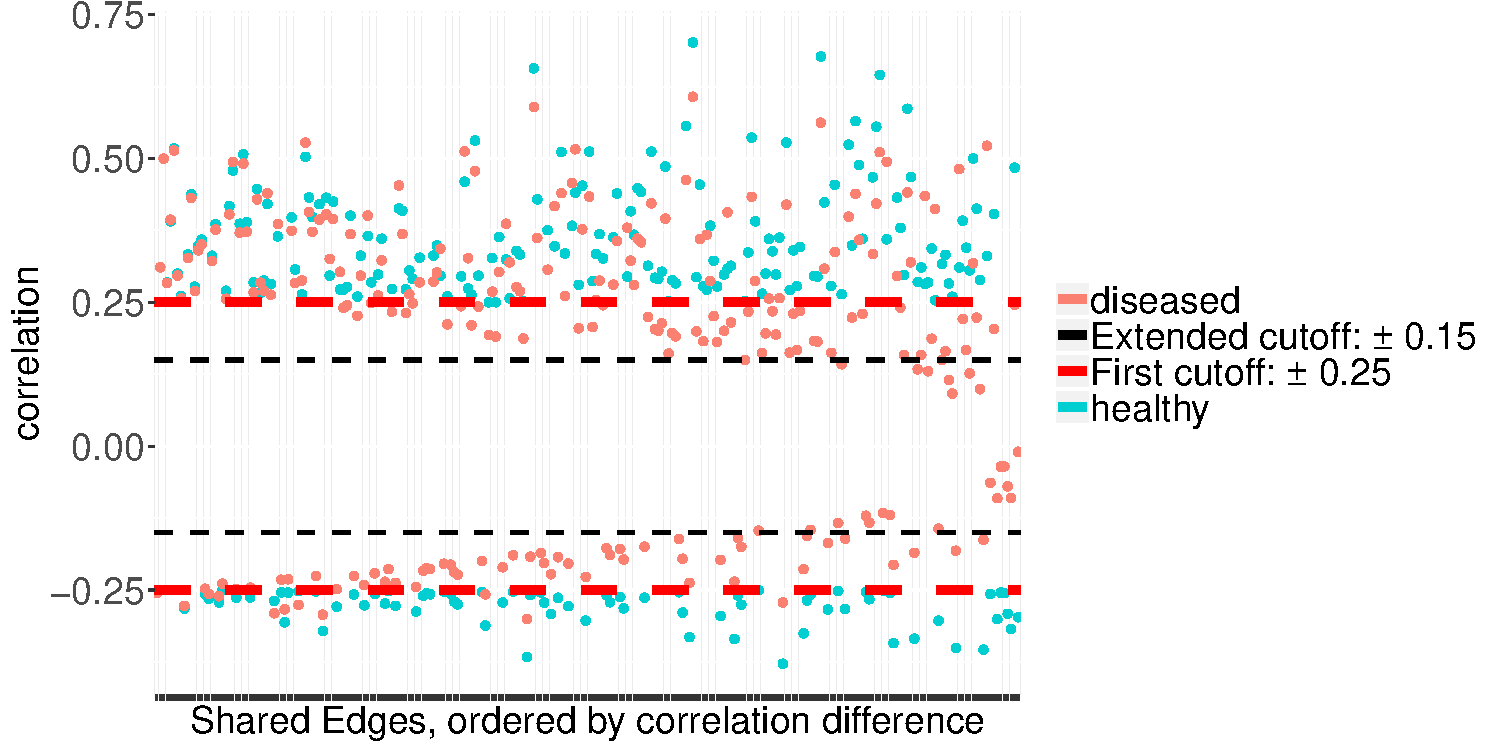
\includegraphics[width=0.95\linewidth]{figure/results/correlation_comparison_h_0_25.pdf}}
%     \caption[Correlation comparisons for the filtered healthy network and the unfiltered diseased network.]{Correlation comparisons for the filtered healthy network and the unfiltered diseased network. Included in this figure are the correlation cutoff value of 0.25 and the extended correlation threshold of 0.15 which is attributed to an extended correlation value of 0.1.}
%     \label{fig-cor-comp-h}
% \end{figure}
% \begin{figure}[!hbt]
%     \centering
%     \fbox{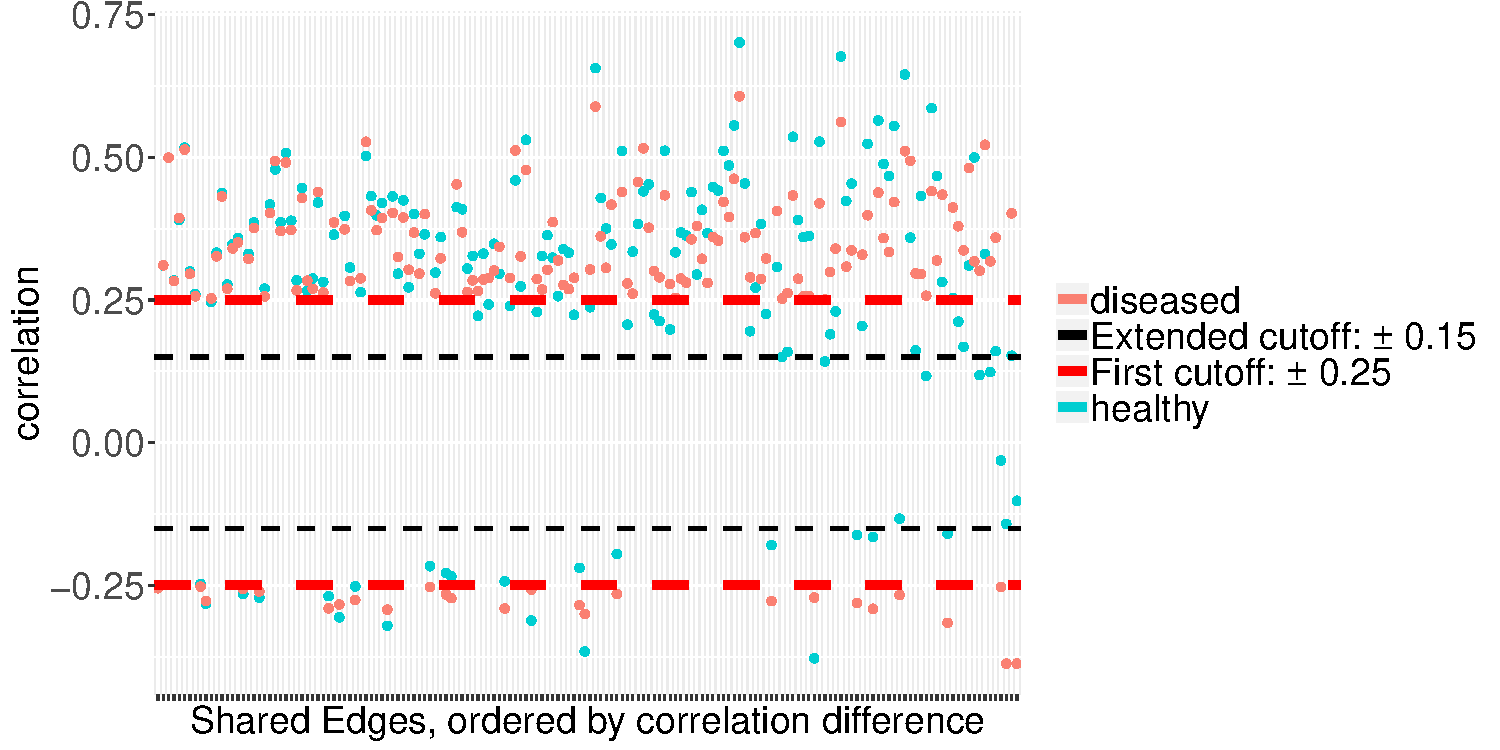
\includegraphics[width=0.95\linewidth]{figure/results/correlation_comparison_d_0_25.pdf}}
%     \caption[Correlation comparisons for the filtered diseased network and the unfiltered healthy network.]{Correlation comparisons for the filtered diseased network and the unfiltered healthy network. Included in this figure are the correlation cutoff value of 0.25 and the extended correlation threshold of 0.15 which is attributed to an extended correlation value of 0.1.}
%     \label{fig-cor-comp-d}
% \end{figure}
\begin{figure}[!hbt]
\centering
\subfloat[Correlation comparisons for the filtered healthy network and the unfiltered diseased network.]{
    \label{subfig:fig-cor-comp-h}
    \fbox{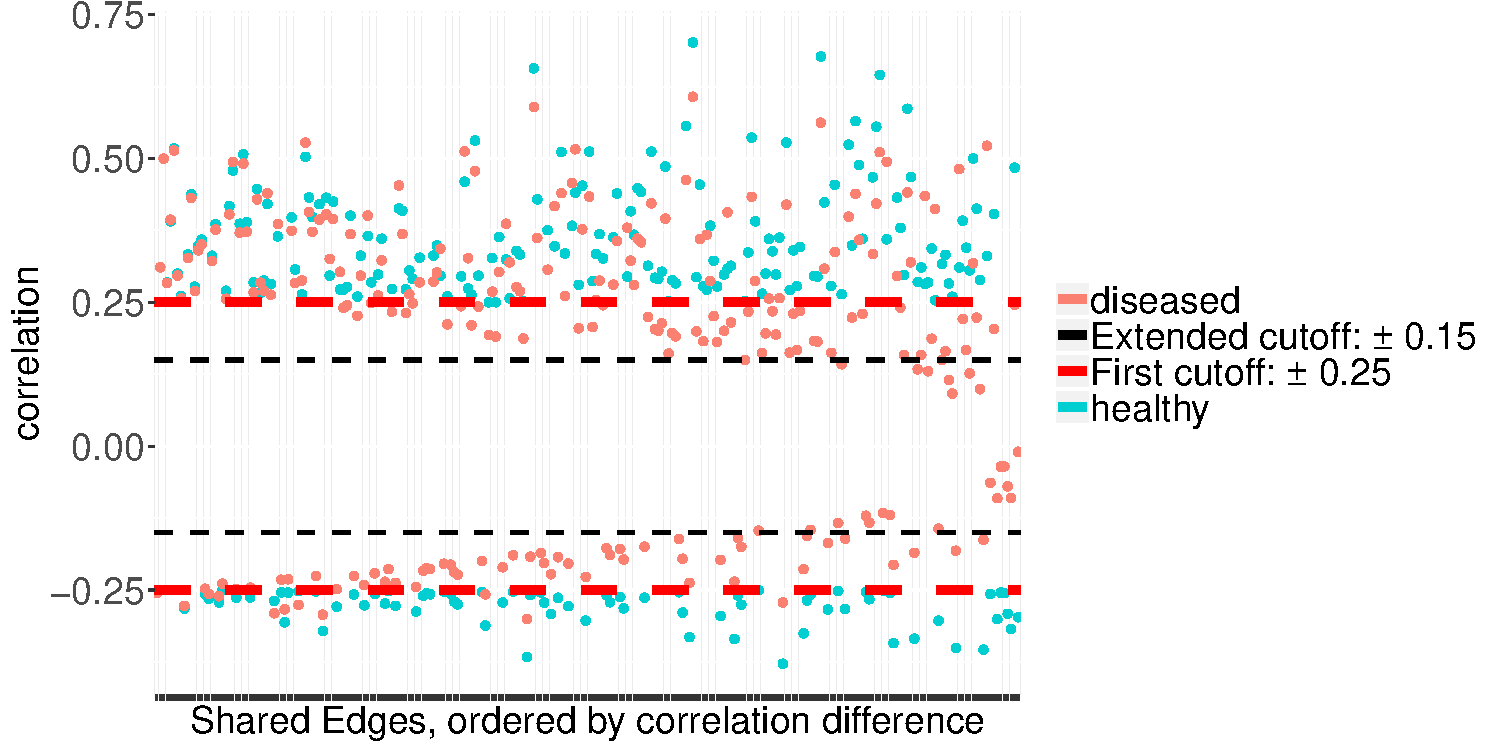
\includegraphics[width=0.95\linewidth]{figure/results/correlation_comparison_h_0_25.pdf}}}
    \hfill
\subfloat[Correlation comparisons for the filtered diseased network and the unfiltered healthy network.]{
    \label{subfig:fig-cor-comp-d}
    \fbox{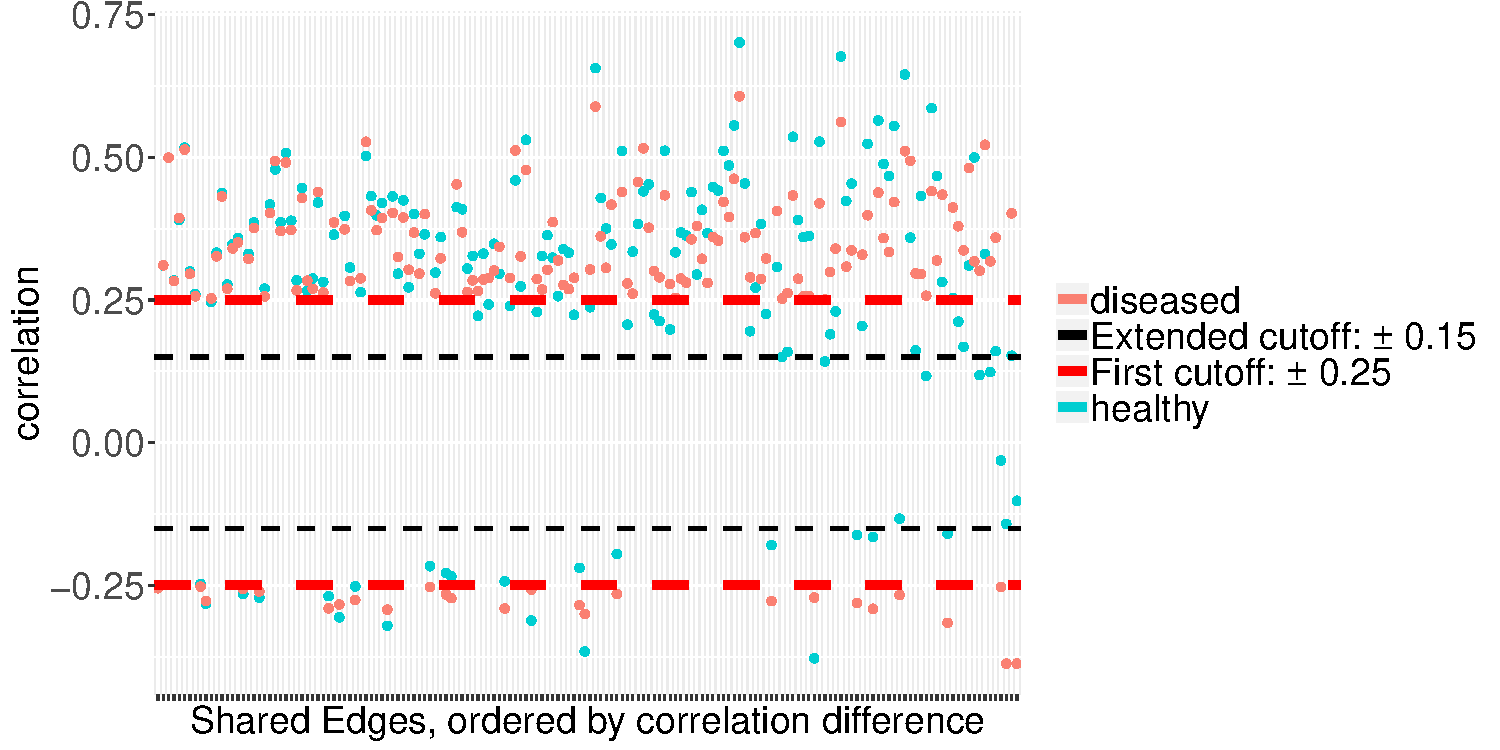
\includegraphics[width=0.95\linewidth]{figure/results/correlation_comparison_d_0_25.pdf}}}
\caption{Correlation comparisons for the filtered and unfiltered networks. Included in this figure are the correlation cutoff value of 0.25 and the extended correlation threshold of 0.15 which is attributed to an extended correlation value of 0.1.}
\label{fig:fig-cor-comp}
\end{figure}

\begin{table}[!btp]
\centering
\begin{tabular}{p{0.1\textwidth} p{0.1\textwidth} p{0.24\textwidth} p{0.24\textwidth} p{0.15\textwidth}}
% \begin{tabular}{p{1.5cm} p{1cm} p{3.5cm} p{3.5cm} p{2.25cm}}
  \toprule
 Cohort Data & Unique Edges & Overlapping Edges: Remaining Filter 1 & Overlapping Edges: Added from Filter 2 & Total Edges: Filter 1 \& 2\\ 
 \midrule
 Healthy & 4753 & 250 &  34 & 306 \\ 
 Diseased & 4753 & 162 & 107 & 313 \\ 
  \bottomrule
\end{tabular}
\caption[Table including the total overlapping edges before filtering, total overlapping edges in each respective network after the first filter, the overlapping edges that were included from the second filter step, and the total edges resulting from both filtering steps.]{Table including the total overlapping edges before filtering, total overlapping edges in each respective network after the first filter, the overlapping edges that were included from the second filter step, and the total edges resulting from both filtering steps. The last column contains the number of edges identified from the filtering method.}
\label{tab:edge_table2}
\end{table}
After experimenting with various extended threshold values, we extended the threshold by a value of 0.1 by considering an extended threshold value of $|c| \geq 0.15$. The implemented version of the normal cutoff value and the extended cutoff for the filtered healthy network is visible in Figure \ref{subfig:fig-cor-comp-h}. Once again the shared edges are sorted by the correlation difference between the healthy and diseased networks. From this plot a majority of the shared edges for the unfiltered diseased network meet the extended cutoff threshold. We use these additional edges in our following analysis for the identification of and comparison of the sub-graphs. 

Table \ref{tab:edge_table2} lists the number of edges associated with this phase of the filtering. For all of the overlapping edges there were 4753 unique edges. Of these there were 250 and 162 remaining after the first filtering step in the healthy and diseased networks respectively. Then after applying the extended correlation threshold, we identified an additional 34 and 107 healthy and diseased respective edges that just missed the initial threshold. These were included in the final networks which ultimately contained a total of 306 and 313 edges respectively.

Using Cytoscape, we generated visual representations of the networks visible in Figures \ref{subfig:healthy-net} and \ref{subfig:diseased-net}. We colored negative correlations blue, positive correlations red, and scaled the thickness of the connections by the edge weights. We include the figures here so that the reader can visualize the resulting networks. The two networks are similar, but do have different structures related to the exclusive edges present. 

\begin{figure}[!hbt]
\centering
\subfloat[Network visualization of the healthy correlation network.]{
    \label{subfig:healthy-net}
    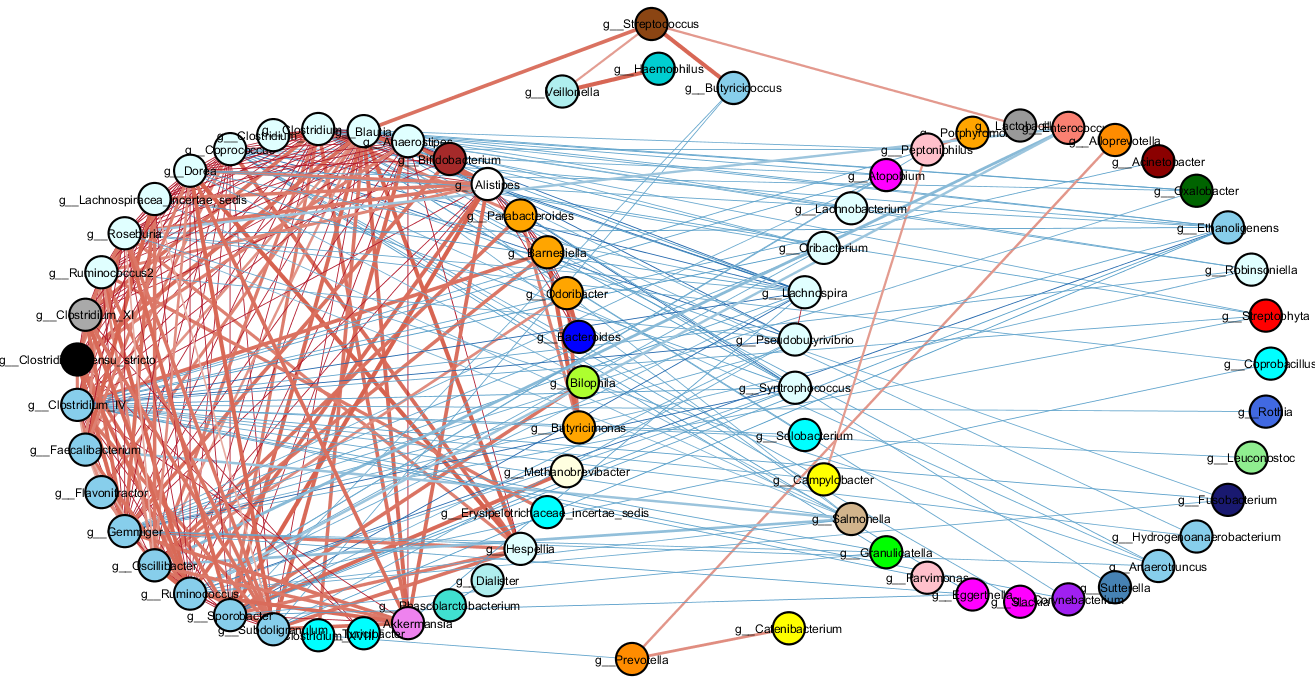
\includegraphics[width=0.85\linewidth]{figure/results/healthy_net.png}}
    \hfill
\subfloat[Network visualization of the diseased correlation network.]{
    \label{subfig:diseased-net}
     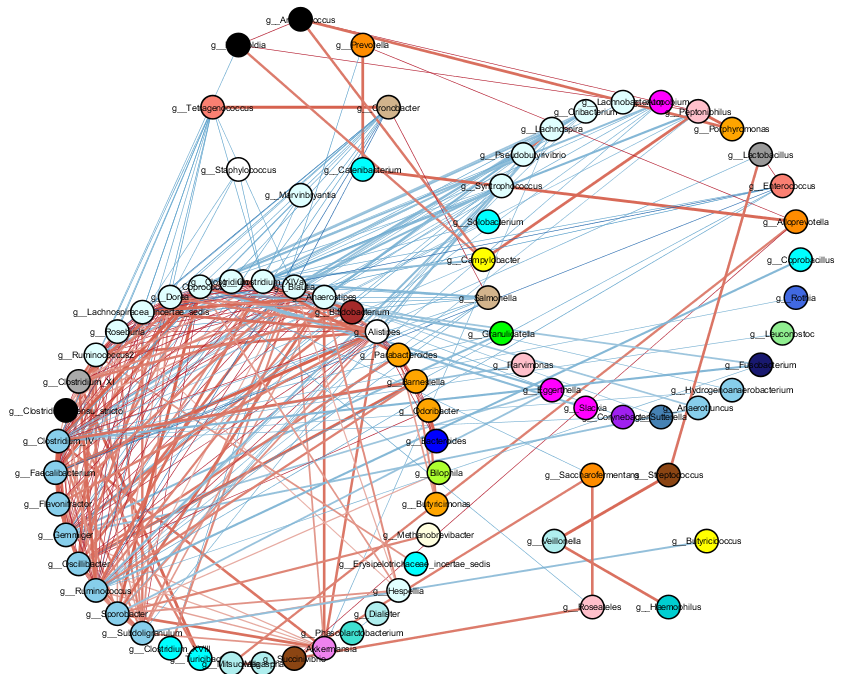
\includegraphics[width=0.85\linewidth]{figure/results/diseased_net.png}}
\caption[Network visualization of the filtered correlation networks.]{Network visualization of the filtered correlation networks. Red indicates positive correlations, blue indicates negative, and the size of the edges is scaled to the correlation value. Taxa are colored by family, and the grouping of the communities is determined by a hierarchical clustering method.}
\label{fig:vis-plots}
\end{figure}

\section{Network Statistics}\label{results-netstat}

The resulting networks generated from the first and second filtering stages resulted in sparsely connected networks with strong correlations. As was discussed previously, the actual network comparisons need to be performed on the overlapping sub-graphs of the two networks. This section presents network statistics of the networks before and after finding the overlapping sub-graphs. 

The filtered healthy network had a total of 306 edges which included 72 unique genera. The remaining genera in this network had at least one edge connecting them to another genus. This was a significant reduction in the number of nodes and connections compared to the original \acrshort{FastSpar} correlation matrix. Originally there were 107 genera that were fully connected with a total number of 5671 unique edges (as presented in Table \ref{tab:edge_table1}). There was a similar reduction in the genera and correlation values with the diseased network. The filtered disease network had a total of 313 edges including 78 unique genera. Once again there was a significant decrease in the number of edges and genera compared to the original network which contained 6105 edges and 111 unique genera.

The intersection of the two networks revealed that there were 67 genera which were present in both networks. This was roughly a quarter of the original genera as there were in the original raw data sets. The healthy sub-graph contained 284 unique edges and the diseased sub-graph contained 269. Of these, the networks shared 261 edges, with there being 23 unique edges in the healthy sub-graph and 8 unique edges in the diseased sub-graph. Despite the small difference in the unique edges, the general network statistics differ. 

\begin{table}[!bt]
\centering
% \begin{tabular}{l p{0.05\textwidth} p{0.05\textwidth} p{0.05\textwidth} p{0.05\textwidth} p{0.12\textwidth}}
\begin{tabular}{l l l l l l l}
  \toprule
 Network & $\overline{k_i}$ & $D$ & $l_G$ & $\overline{C}$ & $\overline{g ( \V )}$  & $\overline{C_{nc}}$ \\ 
  \midrule
Healthy Network (HN) & 8.50 & 0.12 & 2.44 & 0.49 & 53.90 & 5.43 \\ 
  Diseased Network (DN) & 8.03 & 0.10 & 2.77 & 0.49 & 68.22 & 4.96 \\ 
  Sub-graph HN & 8.48 & 0.13 & 2.46 & 0.52 & 50.58 & 5.51 \\ 
  Sub-graph DN & 8.03 & 0.12 & 2.60 & 0.51 & 53.01 & 5.10 \\ 
   \bottomrule
\end{tabular}
\caption[Table containing the general network statistics for the filtered healthy and diseased networks (HN and DN respectively) as well as their sub-graphs.]{Table containing the general network statistics for the filtered healthy and diseased networks (HN and DN respectively) as well as their sub-graphs. The statistics are average degree $\overline{k_i}$,  graph density $D$, average path length $l_G$, average clustering coefficient $\overline{C}$, average betweenness centrality $\overline{g ( \V )}$, and average coreness centrality $\overline{C_{nc}}$. }
\label{tab:netstats}
\end{table}
Table \ref{tab:netstats} contains some of the general network statistics as described in Section \ref{theory-Netshift}. Density values for the sub-graphs appear to be what we would expect from the definition of density. The healthy network does have more edges between the genera, and thus the density is larger due to more of the possible edges existing. The biological interpretation of this would be that the higher the density, the more cross-talk there is between microbes in the network. The healthy network also has a smaller average path length which suggests that the additional edges are connected in key parts of the network that reduce multiple paths. So the smaller the value, the more compact the microbial network is. The average clustering coefficient of the two networks is similar, with the healthy network having a value of 0.52 and the diseased network with a value of 0.51. We would expect that the higher the clustering coefficient, the more independently associated microbes will be present in the network.

The table also contains average values for the degree, betweenness centrality and the coreness centrality. These metrics are important for understanding node level changes in the networks \citep{Kuntal2018}. While we show the average values of the metrics in Table \ref{tab:netstats}, we have included the distribution plots of the values for all of the nodes in the respective networks in the appendix in Figure \ref{fig:dist_plots}. It is evident from Figures \ref{subfig:deg_dist}, and \ref{subfig:btween_dist} that many genera have low degrees and betweenness centrality, but there are several genera with higher values. We would expect higher degrees to be associated with higher importance due to the increased number of direct connections between members of the community. Additionally, higher betweenness centrality highlights the importance as a preferred member of the community. The coreness centrality described in Figure \ref{subfig:core_dist} reveals that there are several genera with a low coreness centrality, and many with higher coreness centrality scores. This indicates that these individuals might have better colony forming capabilities due to the large sub-graphs that can be made with them. We consider these individuals as core areas of the network that are in a core hub community \citep{Kuntal2018}.


After comparing the networks, there are some differences in the taxa associated with the highest degrees, betweenness centrality, and coreness centrality.

We present all of these metrics in the appendix as Table \ref{tab:node-measures}. For the degrees, note that the overlapping networks contain the same top five nodes with respect to degree, even though they have slightly different degree values. This emphasizes the re-wiring that is taking place in the network. If we compare the full networks to the overlapping networks, we find that the healthy network contains four of the same genera, with \textit{g\_Gemmiger} and \textit{g\_Ruminococcus} substituting for each other. In the diseased network we see that the genera are all conserved, with a reduction in the degrees. 

For betweenness centrality three out of the five genera are in the top five between the overlapping networks. \textit{g\_Oscillibacter} and \textit{g\_Sporobacter} are replaced by \textit{g\_Faecalibacterium} and \textit{g\_Coprococcus}. Again, this reveals the change in network wiring. Four out of five genera are conserved from the full healthy network to the overlapping healthy network, and the genera are conserved in the diseased networks. Coreness centrality ranks are the same in the overlapping networks, with the values all being 12 and 11 for the healthy and diseased networks respectively. The healthy network has conserved the genera between the full network and the overlapping network, and the diseased network conserves four out of the five genera. 

\section{Network Structure}\label{res:shift}
For the final results we used \citeauthor{Kuntal2018}'s web application to visualize community structure and identify the driving nodes in the networks. First we present the visualizations of the re-wiring of the networks with the shuffle plot that is used by \citeauthor{Kuntal2018}. The aim of a shuffle plot is to visualize the re-wirings and the subsequent re-grouping of the nodes in the networks. The NetShift method uses a hierarchical clustering algorithm to identify communities within each network. It then looks across the two networks to determine the re-wiring based upon the nodes and the communities they were clustered into in each respective network.
\begin{figure}[!thbp]
    \centering
    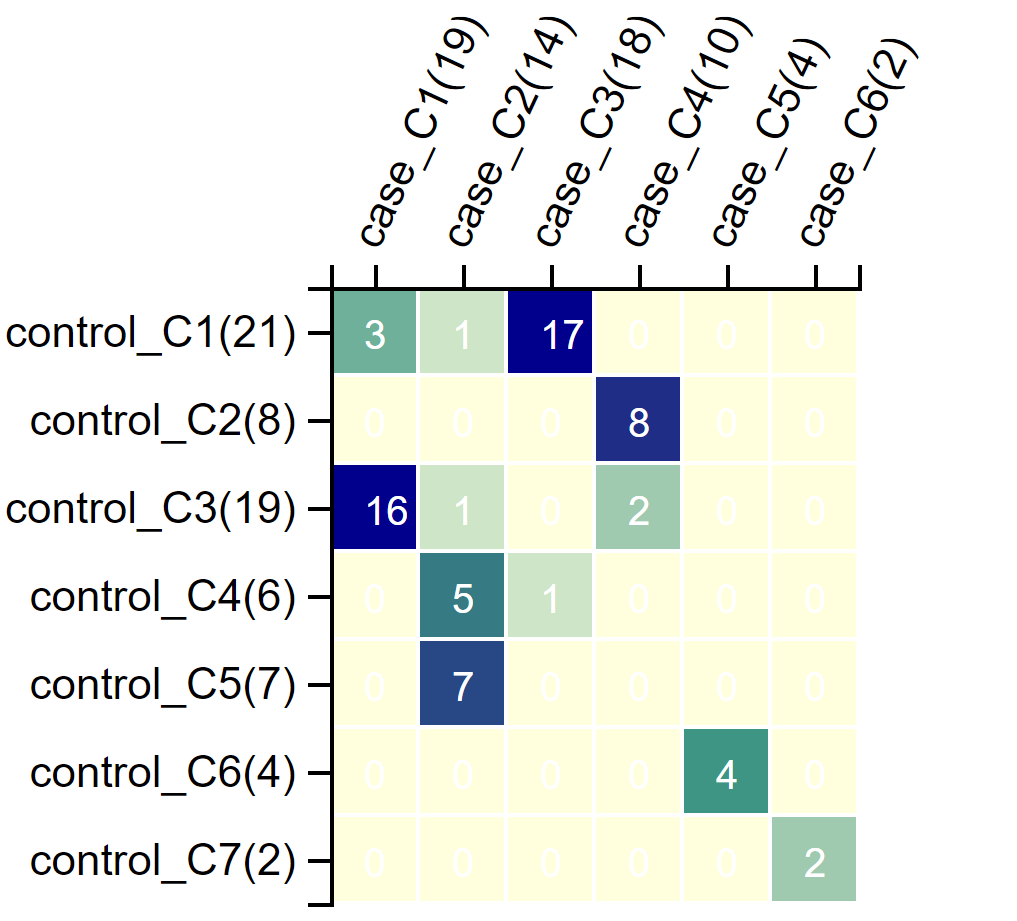
\includegraphics[width=0.8\linewidth]{figure/results/shuffle_plot.png}
    \caption[NetShift shuffle plot indicating community-level structure changes.]{NetShift shuffle plot indicating community-level structure changes.}
    \label{fig:res-shuffle}
\end{figure}
Figure \ref{fig:res-shuffle} depicts the community-level structure changes between the healthy (control) and diseased (case) networks. The plot is interpreted by observing the label for either the control or case network, and the given number in parentheses. The given number defines the amount of genera present in the respective community in the respective network. So, for example, of the 21 genera in \textit{case\_C2(14)}, 1 is located in \textit{control\_C1(21)}, 1 is located in \textit{control\_C3(19)}, 5 are located in \textit{control\_C4(6)} and 7 are in \textit{control\_C5(7)}. Among these genera there is considerable network re-wiring. On the other hand, consider \textit{case\_C5(4)}. All of the genera associated with it in the control network stay together in the same community (\textit{control\_C6(4)}) in the diseased network. Therefore, the more variance across a row or column, the more different the community structure is.  

We have included the network shuffle plot visualization generated from \citeauthor{Kuntal2018}'s tool. Considering the shuffle plot in Figure \ref{fig:res-shuffle}, the network diagram in Figure \ref{fig:res-high} is used to visualize the healthy community placements of the genera associated with the diseased community \textit{case\_C2(14)}.
\begin{figure}[htb!]
    \centering
    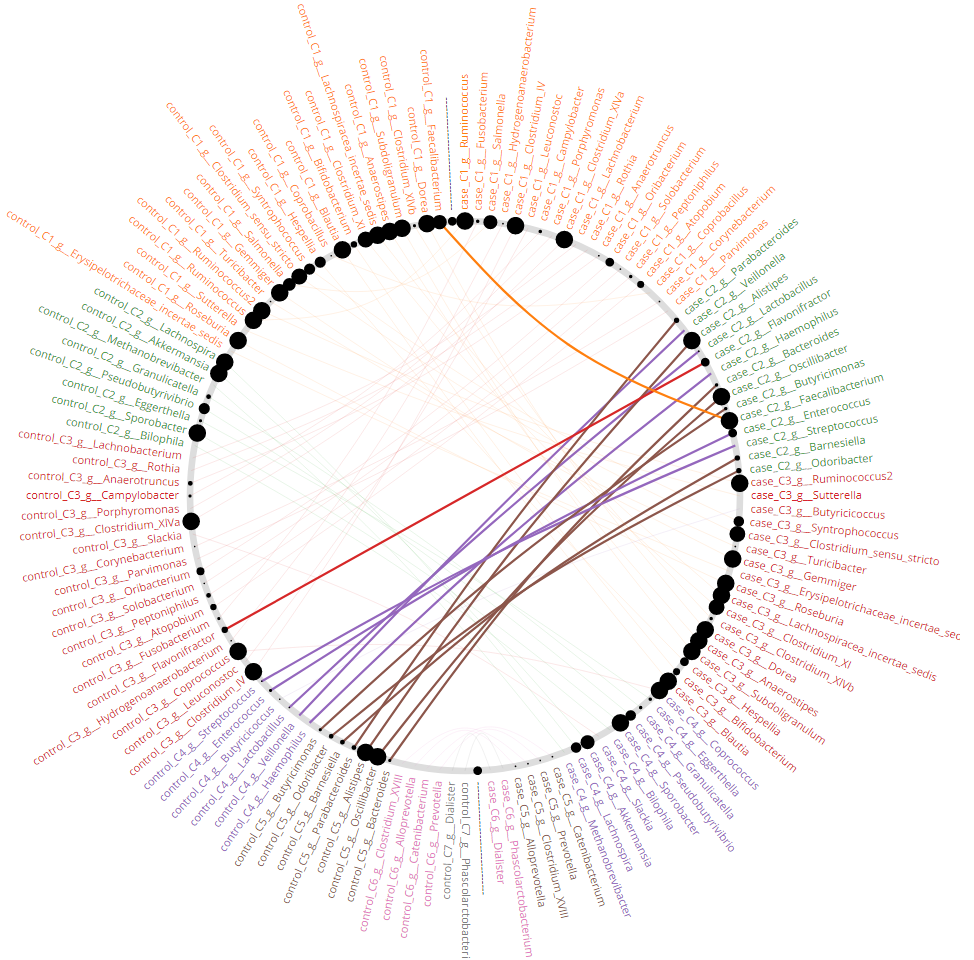
\includegraphics[width=1.0\linewidth]{figure/results/rewire_network.png}
    \caption[The NetShift shuffle diagram highlighting high re-wiring between communities identified by hierarchical clustering.]{The NetShift shuffle diagram highlighting high re-wiring between communities identified by hierarchical clustering. Here we highlight the case community \textit{case\_C2(14)} and the variation in the respective nodes diseased communities. All taxa are represented by the control taxa on the left of the diagram, and case taxa on the right. Hierarchical cluster communities are identified by the color of the taxa.}
    \label{fig:res-high}
\end{figure}
\begin{figure}[htb!]
    \centering
    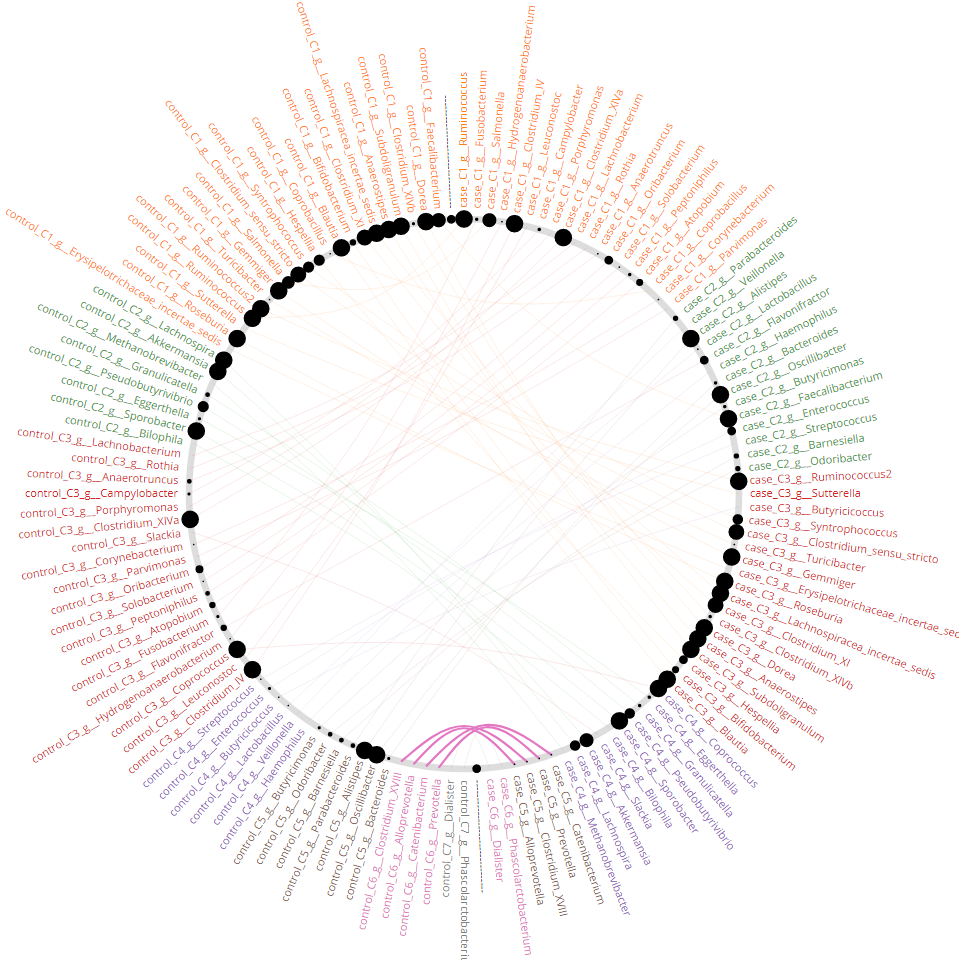
\includegraphics[width=1.0\linewidth]{figure/results/no_rewire_network.png}
    \caption[The NetShift shuffle diagram highlighting low re-wiring between communities identified by hierarchical clustering.]{The NetShift shuffle diagram highlighting low re-wiring between communities identified by hierarchical clustering. Here we highlight the control community \textit{case\_C5(4)} and the conservation of nodes between healthy and diseased. All taxa are represented by the control taxa on the left of the diagram, and case taxa on the right. Hierarchical cluster communities are identified by the color of the taxa.}
    \label{fig:res-low}
\end{figure}
Similarly, Figure \ref{fig:res-low} presents a visualization of the diseased community \textit{case\_C5(4)}. In the diagrams we can follow the lines to see how a taxon may shift communities between the healthy and diseased state. The full diagram is included in Figure \ref{apdx-nesh-shuffle}.

\section{Network Shift}\label{res:netshift}

The \acrfull{JEI} of the overlapping sub-graphs was 0.894, and this score avoids the bias that would have been present had we compared the full networks. To take into account the directionality of re-wiring we utilized the NetShift method and identified several ``driving'' taxa in the networks. These taxa were associated with re-wiring in the network due to their large \acrshort{NESH} and betweenness values.
\begin{table}[!hbt]
\centering
\begin{tabular}{lllll}
\toprule
Genus & Degree (H) & Degree (D)  & Exclusive (D) &\acrshort{NESH}\\
\midrule
g\_Alloprevotella & 1 & 2 & 1 & 1.029\\
g\_Catenibacterium & 1 & 2 & 1 & 1.029\\
g\_Enterococcus\textsuperscript{*} & 4 & 7 & 3 & 0.943\\
g\_Lactobacillus\textsuperscript{*} & 2 & 3 & 1 & 0.695\\
g\_Butyricicoccus & 3 & 1 & 0 & 0.667\\
g\_Anaerotruncus & 4 & 2 & 0 & 0.5\\
g\_Coprobacillus & 2 & 1 & 0 & 0.5\\
g\_Lachnospira & 14 & 7 & 0 & 0.5\\
g\_Streptococcus & 4 & 2 & 0 & 0.5\\
g\_Faecalibacterium\textsuperscript{*} & 12 & 15 & 3 & 0.486\\
g\_Flavonifractor\textsuperscript{*} & 5 & 6 & 1 & 0.362\\
g\_Barnesiella\textsuperscript{*} & 6 & 7 & 1 & 0.314\\
g\_Granulicatella & 4 & 3 & 0 & 0.25\\
g\_Hespellia & 8 & 6 & 0 & 0.25\\
g\_Alistipes\textsuperscript{*} & 19 & 21 & 2 & 0.248\\
g\_Dorea\textsuperscript{*} & 23 & 21 & 1 & 0.237\\
g\_Sporobacter & 23 & 18 & 0 & 0.217\\
g\_Lachnospiracea\_inc.\textsuperscript{*}& 16 & 16 & 1 & 0.205\\
g\_Akkermansia & 12 & 10 & 0 & 0.167\\
g\_Peptoniphilus\textsuperscript{*} & 6 & 5 & 0 & 0.167\\
  \bottomrule
\end{tabular}
\caption[Table containing the top 20 genera with the highest \acrshort{NESH} scores and their respective degree and edge information.]{Table containing the top 20 genera with the highest \acrshort{NESH} scores and their respective degree and edge information. Taxa identified as drivers from the betweenness score and high \acrshort{NESH} score are denoted by a \textsuperscript{*} next to their name. Included in the table are the degrees of the respective genus in the \acrfull{H} and \acrfull{D} network, the intersect (shared edges), the exclusive edges in the case network, and the \acrshort{NESH} score. \textit{g\_Lachnospiracea\_inc.} was abbreviated from: \textit{g\_Lachnospiracea\_incertae\_sedis}. }
\label{tab:nesh}
\end{table}
Table \ref{tab:nesh} lists the top 20 genera sorted by their \acrshort{NESH} scores. The especially important drivers are identified by higher \acrshort{NESH} and betweenness scores from the healthy to the diseased network. Note that it is not required for driving genera to have exclusive edges (as evident for \textit{g\_Peptoniphilus}) because of \acrshort{NESH}'s dependence upon the neighbors of a node. It is also apparent that high \acrshort{NESH} scores are not dependent upon high exclusivity or degrees of a node.

We visualized the drivers and edges in the sub-graph networks in Figures \ref{fig:res-case-only} and \ref{fig:res-control-only} with \citeauthor{Kuntal2018}'s web application.
\begin{figure}[htb!]
    \centering
    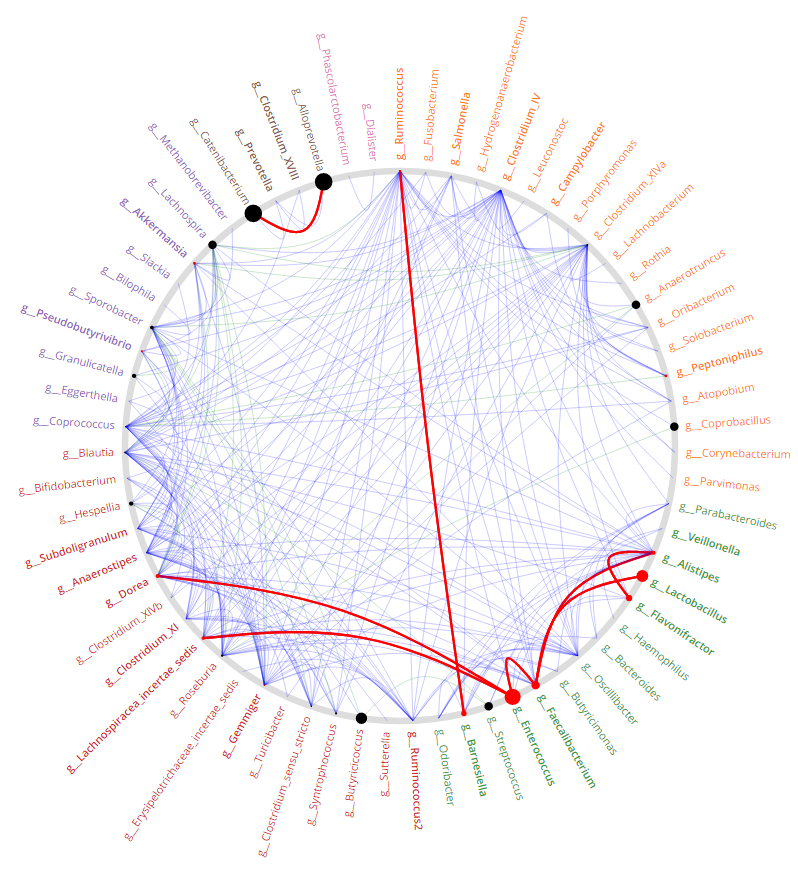
\includegraphics[width=1.0\linewidth]{figure/results/case_only.png}
    \caption[NetShift diagram depicting all edges in the sub-graphs with the diseased-only edges highlighted in red.]{NetShift diagram depicting all edges in the sub-graphs with the diseased-only edges highlighted in red. Genera are colored by their assigned sub-communities. Nodes are scaled by their \acrshort{NESH} scores, and nodes are colored red if they have been identified as important drivers. Control-only edges are in green, case-only edges are in red, and shared edges are in blue.}
    \label{fig:res-case-only}
\end{figure}
\begin{figure}[htb!]
    \centering
    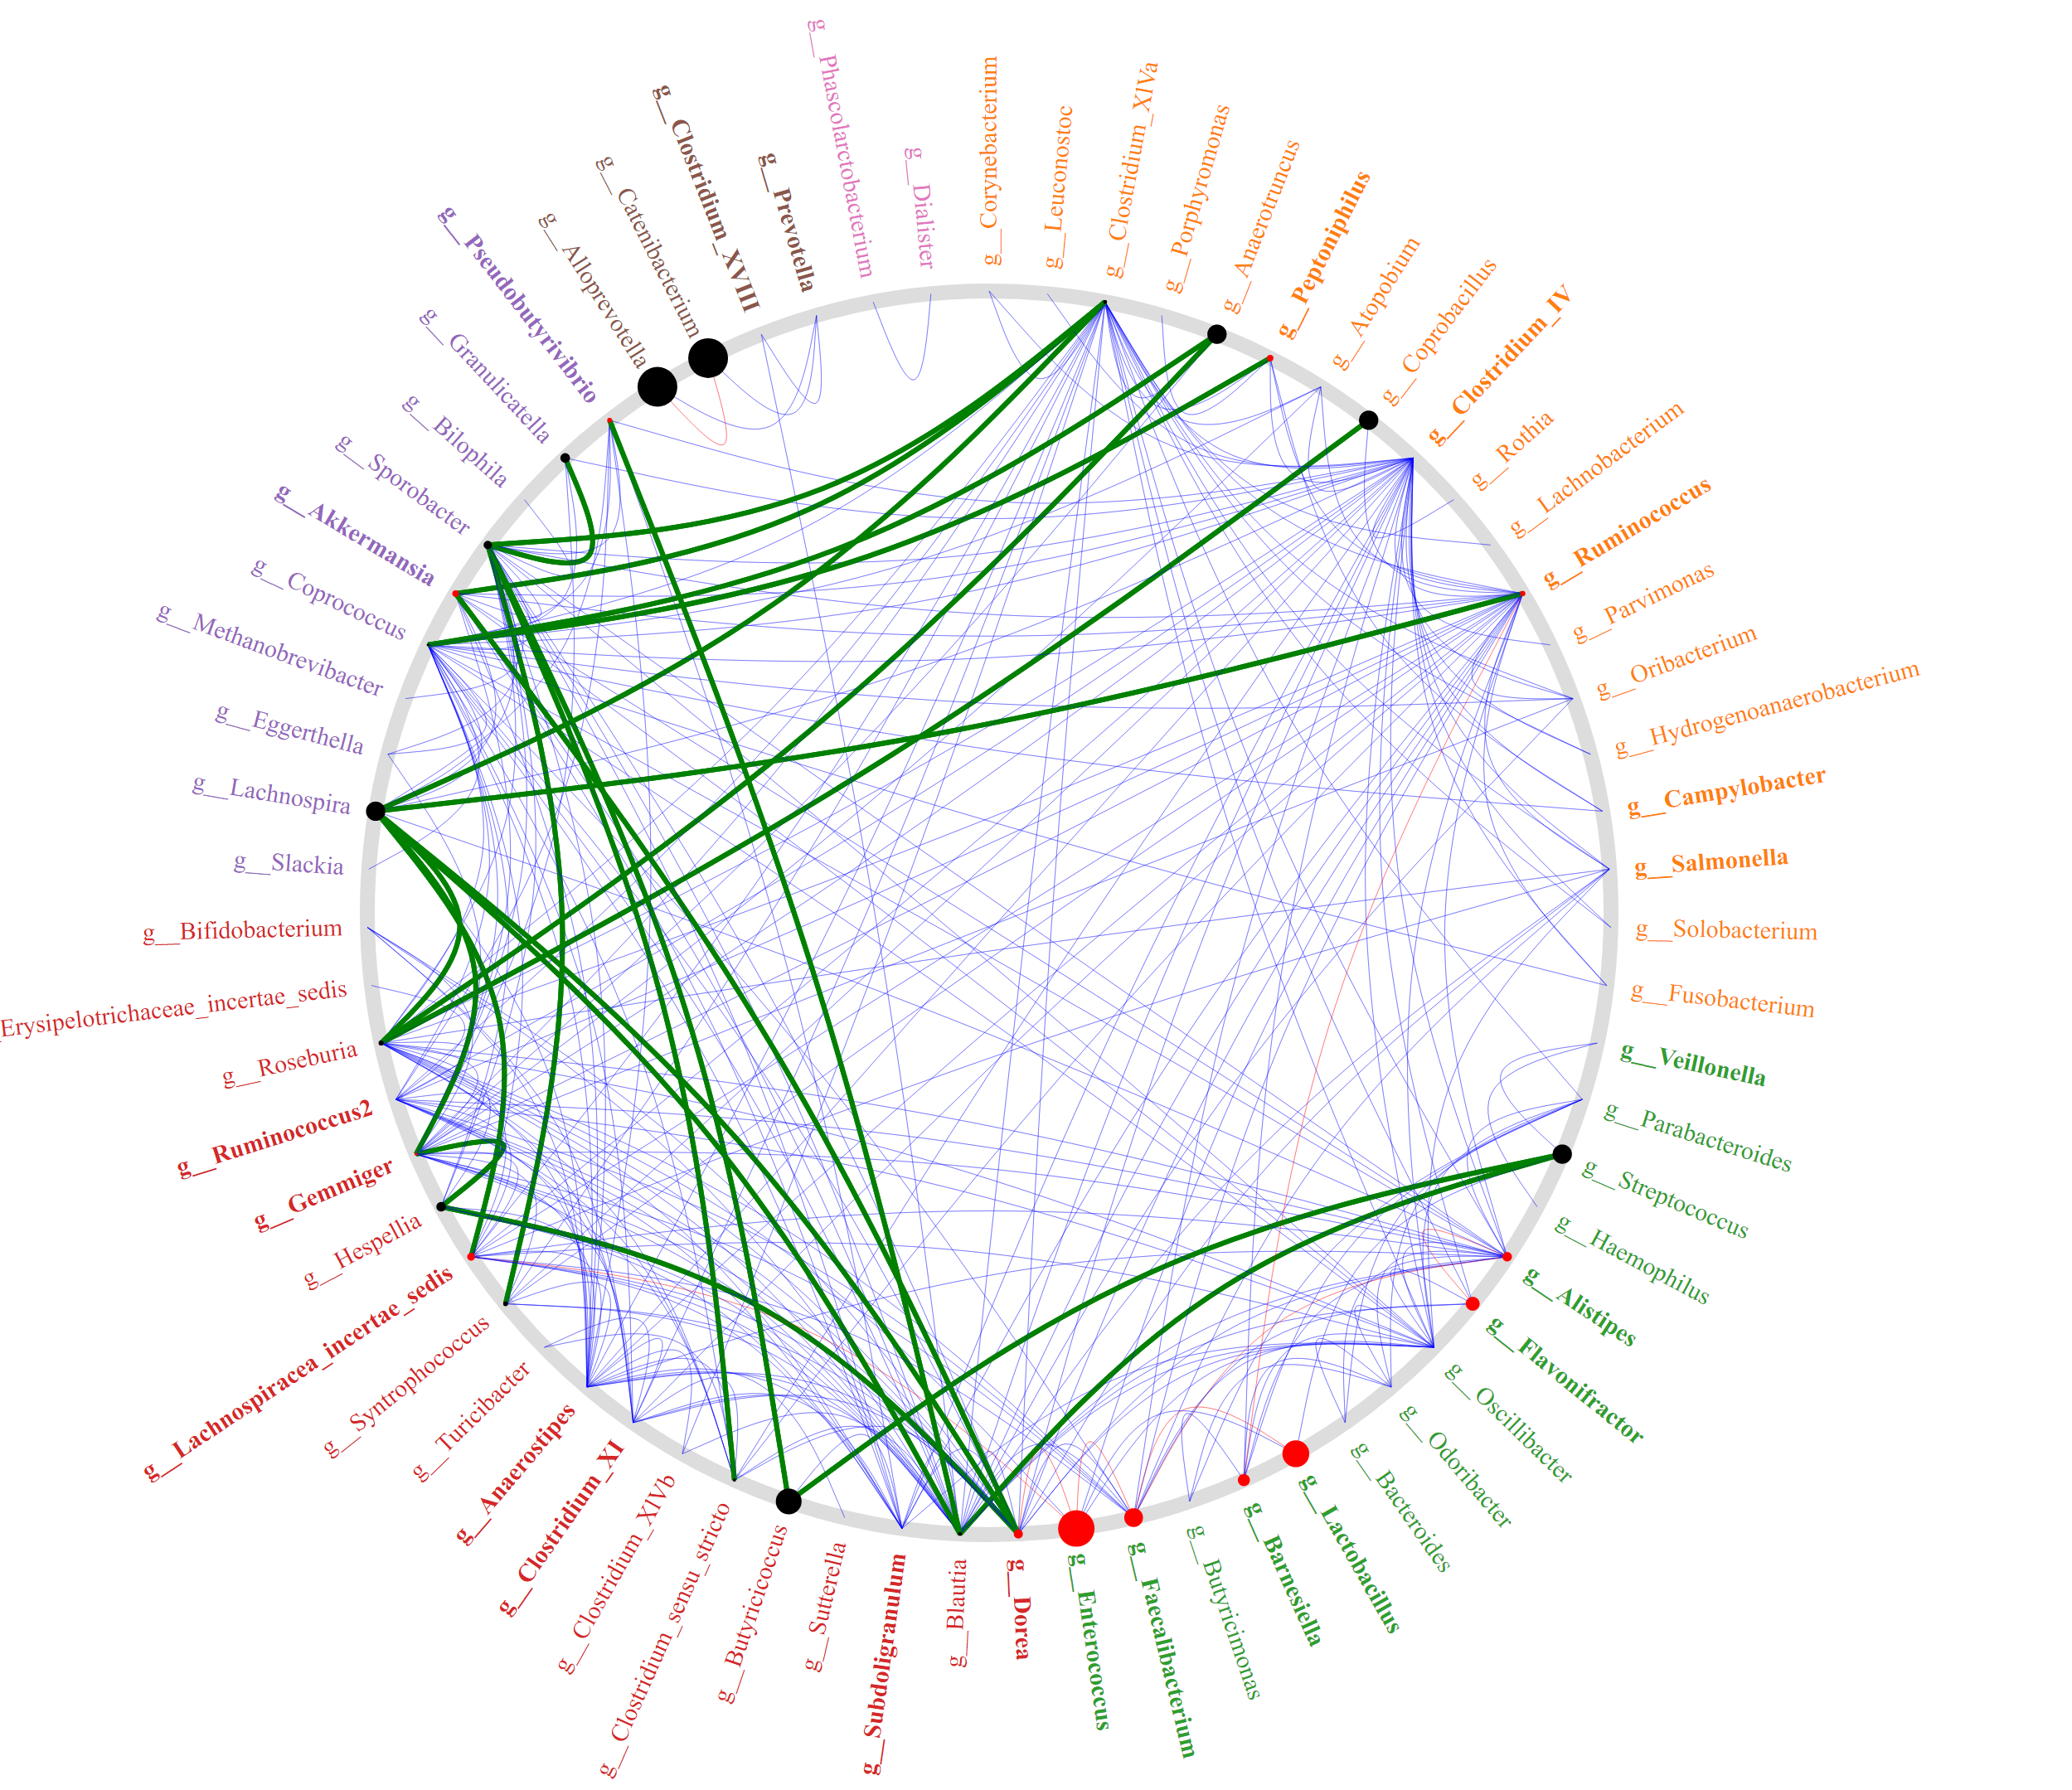
\includegraphics[width=1.0\linewidth]{figure/results/control_only.png}
    \caption[NetShift diagram depicting all edges in the sub-graphs with the control-only edges highlighted in green.]{NetShift diagram depicting all edges in the sub-graphs with the control-only edges highlighted in green. Genera are colored by their assigned sub-communities. Nodes are scaled by their \acrshort{NESH} scores, and nodes are colored red if they have been identified as important drivers. Control-only edges are in green, case-only edges are in red, and shared edges are in blue.}
    \label{fig:res-control-only}
\end{figure}
These figures represent diseased exclusive edges highlighted in red and healthy exclusive edges in green. Both plots use the case network's hierarchical clustering for the ordering and coloring of the names of the taxa. These plots give further evidence of different structure in the healthy and diseased networks due to the exclusive edges and their influence on the hierarchical clustering and re-wiring of network connections discussed in Section \ref{res:shift}. 

With the nodes being scaled according to a genus's \acrshort{NESH} score, and drivers (nodes) colored red, we see the diseased-only edges are primarily connected to driving nodes in Figure \ref{fig:res-case-only}. Additionally, in Figure \ref{fig:res-control-only}, the exclusive healthy edges are connected to many genera that are not defined as drivers. We would expect this result since we are trying to identify taxa that are drivers in the diseased network. 

In order for a node to be designated a driver it had to have a high \acrshort{NESH} score and a positive delta betweenness. Table \ref{tab:nesh-btwn} contains the top 20 \acrshort{NESH} score genera and their delta betweenness between the healthy network and the diseased networks. The identified drivers in Table \ref{tab:nesh-btwn} all have positive betweenness whereas the genera that were not identified had negative delta betweenness values. 

\begin{table}[!hbt]
\centering
\begin{tabular}{lll}
\toprule
Genus & \acrshort{NESH} & $\Delta$ Betweenness\\
\midrule
g\_Alloprevotella & 1.029 &	0\\
g\_Catenibacterium & 1.029 &	0\\
g\_Enterococcus\textsuperscript{*} & 0.943 &	0.005\\
g\_Lactobacillus\textsuperscript{*} & 0.695 &	0.385\\
g\_Butyricicoccus & 0.667 &	-0.018\\
g\_Anaerotruncus & 0.5 &	0\\
g\_Coprobacillus & 0.5 &	0\\
g\_Lachnospira & 0.5 &	-0.003\\
g\_Streptococcus & 0.5 &	-0.046\\
g\_Faecalibacterium\textsuperscript{*} & 0.486 &	0.427\\
g\_Flavonifractor\textsuperscript{*} & 0.362 &	0.001\\
g\_Barnesiella\textsuperscript{*} & 0.314 &	0.018\\
g\_Granulicatella & 0.25 &	0\\
g\_Hespellia & 0.25 &	0\\
g\_Alistipes\textsuperscript{*} & 0.248 &	0.027\\
g\_Dorea\textsuperscript{*} & 0.237 &	0.033\\
g\_Sporobacter & 0.217 &	-0.087\\
g\_Lachnospiracea\_incertae\_sedis\textsuperscript{*}& 0.205 &	0.019\\
g\_Akkermansia & 0.167 &	0.004\\
g\_Peptoniphilus\textsuperscript{*} & 0.167 &	0.002\\

  \bottomrule
\end{tabular}
\caption[Table containing the identified drivers from the top 20 \acrshort{NESH} scores.]{Table containing the identified drivers from the top 20 \acrshort{NESH} scores and their related delta betweenness score from control to case. Taxa identified as drivers from the betweenness score and high \acrshort{NESH} score are denoted by a \textsuperscript{*} next to their name.}
\label{tab:nesh-btwn}
\end{table}
Considering these top 20 \acrshort{NESH} scores and delta betweenness values, the NetShift methodology identified \textit{g\_Enterococcus}, \textit{g\_Lactobacillus}, \textit{g\_Faecalibacterium}, \textit{g\_Flavonifractor}, \textit{g\_Barnesiella}, \textit{g\_Alistipes}, \textit{g\_Dorea},
\textit{g\_Peptoniphilus}, and  \textit{g\_Lachnospiracea \_incertae\_sedis} as drivers in the diseased state. These metrics suggest that the identified genera play some role in the re-wiring of the network from a healthy to diseased state.
